\documentclass[11pt]{article}

\usepackage{sectsty}
\usepackage{graphicx}
\usepackage{multirow}
\usepackage{abstract}

\renewcommand{\contentsname}{\centering Contents}   
\renewcommand{\abstractnamefont}{\normalfont\normalsize\bfseries\Large}
\renewcommand{\abstracttextfont}{\large}

% Margins
\topmargin=-0.45in
\evensidemargin=0in
\oddsidemargin=0in
\textwidth=6.5in
\textheight=9.0in
\headsep=0.25in

\title{Monte Carlo Tree Search driven Falsification}
\author{Lugi Berducci \and Alessandro Steri}
\date{\today}

\begin{document}
\maketitle	


%--Paper--
\begin{abstract}
Simulation-based verification is often the only chance to verify complex hybrid systems and it requires a large amount of time and resources.
In particular, the process to find anomalies and faults is called \textit{falsification} because it consists of finding a scenario (a trace of disturbances) that lead the system to falsify the requirements, described as formal specifications.

Many research groups are focusing their effort on techniques for reduction of verification time and recent works adopted search algorithm driven by a heuristic called \textit{robustness}.

In this project, we focused on falsification of Temporal Logic Specification using one of the most promising search algorithm: the Monte Carlo Tree Search, famous for being adopted in AlphaGo. Specifically, we tested this approach on the well-known Automatic Transmission model and analysed the obtained result, describing strenghts and difficulties of MCTS algorithm.

\end{abstract}

% Optional TOC
\tableofcontents

\pagebreak

\section{Two-Layered Falsification}
\subsection{Introduction}
The process of falsification aims to find a counter example to a given specification, such example typically are \textit{hard to find}  errors. Typically the search space is huge and the process of verification through simulation is quite expensive, thus a clever strategy to drive the search and properly invest the simulation time is essential.

Following the work done in \cite{zhang2018two} we decided to use a two layer strategy. On the top level Monte Carlo Tree Search act as a zoomed out view of the search in which, at each control point, the system quantizes the input space in regions and tries to iteratively explore new regions and give to those region an estimation on how promising they are (see section..). 
On the bottom a generic search algorithm (see section ..) further investigate promising regions at an finer grain coming from the top layer and updates their value of "promisingness" (maybe confidence??).

The MCTS is often used in automated game play (see alphago). This clearly underlines that, in fact, the model we are facing is an adversarial model. As if there was an adversary the error is cleverly placed and the strategy needs to be clever enough to find it. 

The MCTS allow to fine tune the balance between exploration and exploitation at a macroscopic level while the choice of the second layer acts in the same way but atomically over points in the search space.

\subsection{Upper-layer: MCTS}~\label{sec:MCTS}
The MCTS aims to iteratively build a tree $T=(V,E)$ where nodes in $V$ are labelled with a score $s$ and a counter $n$ and edges in $E$ are labelled with actions. At the start the tree is initialized as a root node with $s=Inf$ and $n=0$. The execution evolves in different phases.

\paragraph{Selection:} Starting from the root until reaching a leaf (of the MCTS tree) we move to the node $n$ maximizing UCB($n$) (see ...). 
The leaf, say $L$ will be sampled. If $L$ is sampled for the first time then Rollout($L$), else Expansion($L$).

\paragraph{Expansion:} For each action $a$ available from $L$ we extend $T$ with a new node $v $  with $s=Inf$, $n=0$ and edge label $a$. Then a random child of $L,$ say $C_L,$ is chosen to do Rollout($C_L$).

\paragraph{Rollout(L)} For each ancestor of $L$ starting from the root till $L$ itself, the search algorithm (see section) is run in the region of the selected node. Then starting from L, the rest of the trace is simulated driven by the search. At the end the trace will have a robustness value of $v$ which will be used as an estimate for $L$ and its ancestors by means of Backpropagation($L,v$).

\paragraph{Backpropagation(L,v):} From $L$ till the root, going trough $L$'s ancestors say $L=a_1, a_2, \dots, a_n=root$ , generic $a_i$ is updated incrementing $n$ and setting $s=max\{n.s, v\}$.

i\paragraph{UCB:} In the most general MCTS implementation, given a node $n$ its UCB value is computed as FOO, where the idea behind the parameter $C$ is to fine-tune exploration vs exploitation. When considering the falsification problem thus using robustness as heuristic we face two problem:
\begin{itemize}
    \item Robustness can have positive yet negative values while classical UCB is designed to work with only positive value. 
    \item Generally, given a specification it is not possible to give an upper bound to the robustness domain. 
\end{itemize}
To overcome both the problems, along the line of CITE, we used U.. defined as BAR.

\pagebreak
\begin{itemize}
    \item tree animation gif
\end{itemize}

\subsection{Lower-layer: Search Algorithms}
In the very end, the falsification task boils down to a search in the space of the states. 
We aim to find a falsifying trace of $k$ disturbances, where $k$ is the number of desired control points. 
To do so the MCTS (see Section~\ref{sec:MCTS}) when selects a node at depth $h$ to rollout from it's basically defining a meta-trace $\hat{T}$. The first $h$ meta-disturb of $\hat{T}$ ($\hat{T}$ prefix) are regions of the input space in which to bound the search, and in the suffix the search is allowed in the whole input space. 
One of the following search algorithm is then used to produce a trace $T$ accordingly with the semantic of $\hat{T}$.

different algo to test the sinergy with MCTS and with the falsification in general. also vs overhead
brief explaination of the search algorithms.

\subsubsection{Random Search: MCTS left alone}
To have a way to evaluate the contribution purely given by the MCTS layer, we decided to implement a fast yet dumb search strategy.
Given a meta-trace $\hat{T}$, for each control point $k$ in $\hat{T}$, RS basically samples u.a.r. a disturbance from the appropriate region for such control point.
This result in a very fast yet only exploring algorithm. 

\subsubsection{Hill Climbing: the greedy}
Here, the classical Hill Climbing implementation has been used. The only difference is that, since eventually we need a full trace (a trace having a disturbance for each control point), in the case a not worst neighbour is found a random one is selected. To have a stronger falsification power, at the cost of a longer simulation time restart has been implemented. On the other hand to speed up the simulation, at the cost of a weaker falsification power it is possible to limit the number of
neighbour tested by the algorithm at each step. 
Clearly this search strategy is way clever and effective than RS but the simulation time needed to carry on the falsification process whit a non trivial property to falsify is of another order of magnitude.

\subsubsection{Simulated Annealing: the impatient}
Again, classical search algorithm, basically an HC enriched with a notion of temperature or, as it is in this case, the number of simulated trace. The higher the temperature the hardest is to make a pejorative move. 
The goal here is to further balance exploration and exploitation and be, in terms of speed and performance in the middle of RS ans HC.
\pagebreak

\section{Experimental phase}~\label{sec:exp}
focus on experimental details, which model, which specification, which algorithms adopted.

\subsection{Model and Specifications}~\label{sec:exp:spec}
The benchmark adopted is the Automatic Transmission by MathWorks, provided in Simulink. It models a vehicle equipped with a trasmission controller and allows the user to change two input signals: the     throttle and the brake.

There are several specifications defined on this model because it is a common benchmark in verification papers. Starting from the reference paper and \cite{bardh2014benchmarks}, we selected two           specification:

\begin{enumerate}
    \item The engine speed never reaches 120.
    \item If the vehicle gear is 3 then the speed is always greater than 20.
\end{enumerate}

We selected these two specifications because they are representative of different kind of search. The first one is easier to falsify, compared with the second one.

\subsection{Implementation of Robustness metric}
In order to undestand the difficulty of falsification of the second specification, we need to spend a few words on the computation of robustness metric used to drive the search.

According to the definition of Robustness given in\cite{fainekos2006robustness}, this metric gives us a measure of how the state of the model is far from the falsification. In the first specification,    the computation of Robustness is simply the difference between the reference speed and the current speed. Conversely, in the second specification the computation is more complex and can be summarized by  the following steps:

\begin{enumerate}
\item Since the second specification is an implication, we wrote it as an \texttt{OR}.
\item The Robustness of the \texttt{OR} operator is the max value of the Robustness computed in the two subformulas.
\item The first subformula is the absolute value of the difference between the current gear and the reference gear (3).
\item The second subformula is the difference between the current speed and the reference speed (20).
\end{enumerate}

Notice that the value of the second subformula is positive if the current speed is greater than 20, otherwise is negative. Conversely, the value of the first subformula is a small positive integer.

As a result, when the gear is different from the reference one (3) then the first subformula dominates the Robustness computation. When the gear is the third one, then the value could be dominated by     the second subformula only if it is greater than 20 and then positive. Then, the resulting metric space is characterized by long plateau when the current speed is far from 20 and local minima because of  the different unit of measurement for gear and speed.

\subsection{The proposed baseline: \texttt{URS}}
The two specifications above have been implemented in an external function in order to maintain a single model file. The Simulink model is characterized by two output blocks, respectively the \textit{speed} and the \textit{gear}. The external function computes the robustness according to the specification, described by a parameter in the configuration file.
\\ \\
The second specification S2 caused too long time to reach falsification and we decided to change its implementation in order to make it suitable to the time and resources that we can use. In particular, one of the main problem of S2 is the different units of measurment that lead to local minima. In fact, whilst speed is between 0 and 100, the gear is an integer value between 1 and 4.

In contrast with the original definition of the Robustness, we proposed to normalize the second subformula of S2 according to the unit scale. Since the speed goes from 0 to 100, we normalize the second subformula dividing by 100. In this way, the Robustness metric is still characterized by long plateau which make the search not trivial but we reduced the number of local minima.

\begin{figure}[h]
    \centering
    \textbf{Uniform Random Sampling - Robustness Distribution}\par
    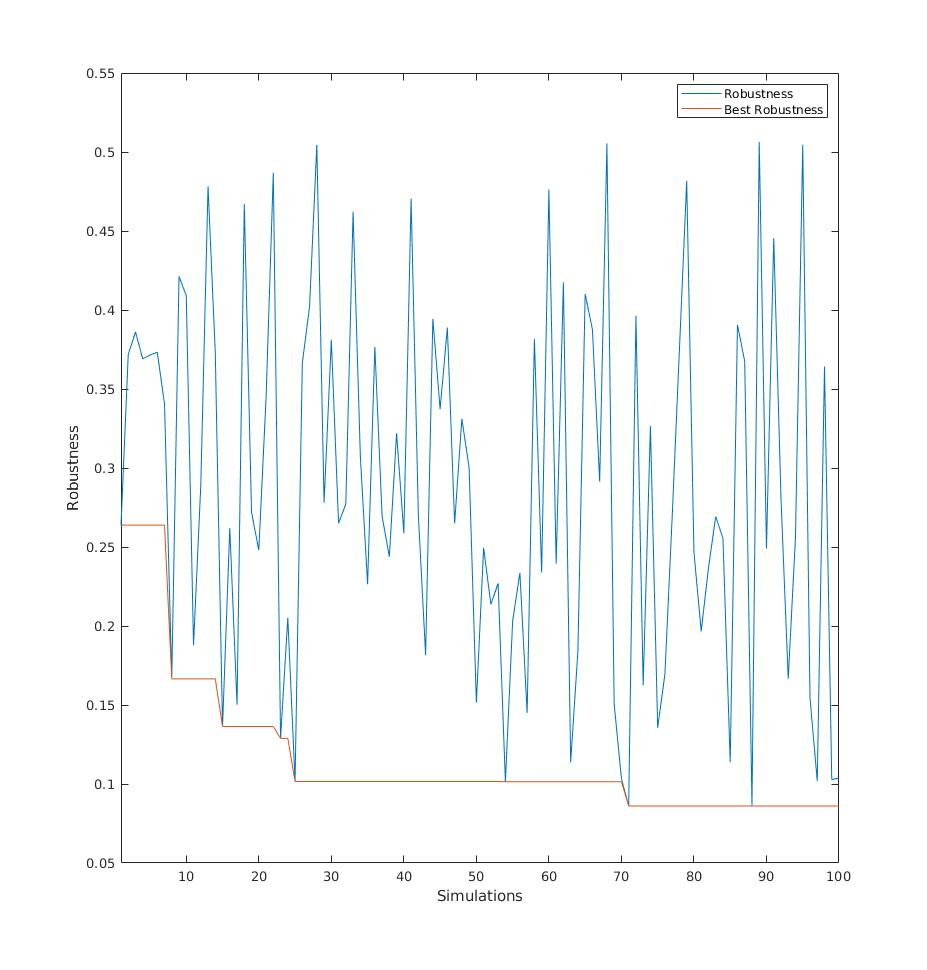
\includegraphics[width=0.5\linewidth]{img/urs_rob_distr.jpg}
    \caption{Robustness distribution over 100 simulation of URS search. This random distribution highlights that there is no learning in URS. Moreover, all the values are in [0,1] because we are using the normalized version of specific \texttt{S2} and is rather likely to reach the third gear at least once during the simulation with random values.}
\end{figure}

\pagebreak

\subsection{Experiments}
In order to evaluate the effectiveness of the proposed falsification framework, we executed a bunch of experiments on the Automatic Transmission model considering several search algorithms: Uniform Random Sampling (URS), MCTS with Random Search (MCTS+RS), MCTS with Hill Climbing (MCTS+HC), MCTS with Simulated Annealing (MCTS+SA).

Since the execution of experiments is based on randomness, we repeated the same experiment 10 times to ensure more confident results.

First of all, we observed that the effectiveness of MCTS is based on its capacity to build the complete tree. In fact, the MCTS algorithm is characterized by a inherent phase of exploration which allows to have a general view of the space (tree width) and the time (tree height). Only when the tree is complete, the MCTS algorithm results effective and specializes the search.
As a consequence, if the branching factor of the nodes is too high, the number of simulation required to build the entire tree is huge and the MCTS doesn't result effective, compared with the URS. 

Thus, in order to exploit the power of MCTS, we tuned the split parameters for the input signals. The Speed signal has been split into 2 regions and the Brake signal has been split into 3 regions, then the branching factor of the tree is 6. In the original paper \cite{zhang2018two}, they
adopted a different tuning but we observed that such tuning is not effective compared with the URS algorithm. Moreover, for reason of time and resources, the experiments below have been configured with budget parameter equal to 100, it means that the maximum number of iterations of MCTS is 100 and then this is an upperbound in the number of simulations.

The tables below [ref] show the obtained results varying the parameter C which balance the value of exploration and exploitation in the UCB formula. The tables contain the following fields:
\begin{itemize}
    \item Algo: Search algorithm adopted.
    \item C: Value of parameter C.
    \item Avg Trace Falsification: Number of trace before falsification, considering only the tests which falsify the specification.
    \item Success Rate: Number of tests which falsify the specification.
    \item Robustness: statistics on robustness value.
    \item Time: statistics on elapsed time, both time are considered as average of the all number of experiments.
\end{itemize}

% TEST ON SPEC 1
\begin{table}[ht]
\centering
\title{Experiments on specification \texttt{S1}}
\begin{tabular}{|l|l|c|c|c|c|c|c|c|}
\hline
\multicolumn{1}{|c|}{\multirow{2}{*}{Algo}} & \multirow{2}{*}{C} & Avg Trace               & \multirow{2}{*}{Success Rate} & \multicolumn{3}{c|}{Robustness} & \multicolumn{2}{c|}{Time (sec)} \\ \cline{5-9} 
\multicolumn{1}{|c|}{}                      &                    & Falsification           &                               & min       & avg      & std dev  & tot        & trace        \\ \hline
URS                                         & - - -              &  40.0                   & 2/10                          & -4.07960  & 4.91882  & 5.514537 &  178.014 &  2.010    \\ \hline
MCTS+RS                                     & 0.500              & - - -                   & 0/10                          &  5.30248  & 8.34921  & 2.400517 &  559.916 &  5.599    \\
MCTS+HC                                     & 0.500              &  94.0                   & 1/10                          & -1.93401  & 5.07959  & 4.386757 & 1034.225 & 10.405    \\
MCTS+SA                                     & 0.500              &  24.0                   & 1/10                          & -0.68394  & 7.71311  & 4.152730 &  891.788 &  9.781    \\ \hline

MCTS+RS                                     & 0.250              &  62.0                   & 4/10                          & -4.52952  &  2.80386 & 4.995340 &  355.163 &  4.198    \\
MCTS+HC                                     & 0.250              &  74.4                   & 5/10                          & -3.63763  &  2.02058 & 4.289398 &  676.262 &  7.774    \\
MCTS+SA                                     & 0.250              &  74.6                   & 7/10                          & -10.29078 & -2.38069 & 3.744391 &  597.866 &  7.297    \\ \hline

MCTS+RS                                     & 0.125              &  46.5                   & 8/10                          & -6.27352  & -1.28520 & 3.320830 &  170.078 &  2.996    \\
MCTS+HC                                     & 0.125              &  68.1                   & 8/10                          & -4.61933  & -0.07330 & 4.719893 &  380.664 &  5.127    \\
MCTS+SA                                     & 0.125              &  48.5                   & 8/10                          & -6.43350  & -0.69363 & 5.875865 &  304.758 &  5.225    \\ \hline

MCTS+RS                                     & 0.000              &  64.5                   & 2/10                          & -4.20689  & 6.83323  & 7.070816 &  325.054 &  3.510    \\
MCTS+HC                                     & 0.000              &  41.0                   & 4/10                          & -2.64884  & 1.95654  & 3.712926 &  430.037 &  5.589    \\
MCTS+SA                                     & 0.000              &  78.0                   & 2/10                          & -1.51834  & 4.81908  & 6.613282 &  558.383 &  5.834    \\ \hline
\end{tabular}
\caption{Comparison between MCTS and URS, given a budget of 100 simulations and varying the parameter C in order to balance exploration and exploitation in the search. The input signals have been split into 2 and 3 region.}~\label{table:res:s1}
\end{table}

% TEST ON SPEC 2
\begin{table}[ht]
\centering
\title{Experiments on specification \texttt{S2}}
\begin{tabular}{|l|l|c|c|c|c|c|c|c|}
\hline
\multicolumn{1}{|c|}{\multirow{2}{*}{Algo}} & \multirow{2}{*}{C} & Avg Trace               & \multirow{2}{*}{Success Rate} & \multicolumn{3}{c|}{Robustness} & \multicolumn{2}{c|}{Time (sec)} \\ \cline{5-9} 
\multicolumn{1}{|c|}{}                      &                    & Falsification           &                               & min      & avg      & std dev  & tot        & trace        \\ \hline
URS                                         & - - -              & - - -                   & 0/10                          & 0.02080  & 0.06130  & 0.03130  &  408.585   &  4.086       \\ \hline
MCTS+RS                                     & 0.500              &  90.0                   & 2/10                          & 0.00000  & 0.05430  & 0.04420  &  397.635   &  4.056       \\
MCTS+HC                                     & 0.500              &  53.0                   & 7/10                          & 0.00000  & 0.00490  & 0.00840  & 1039.426   & 15.517       \\
MCTS+SA                                     & 0.500              & - - -                   & 0/10                          & 0.00071  & 0.04930  & 0.04330  &  681.465   &  6.815       \\ \hline

MCTS+RS                                     & 0.250              & - - -                   & 0/10                          & 0.00661  & 0.03571  & 0.02372  &  572.351   &  5.723       \\
MCTS+HC                                     & 0.250              &  29.1                   & 9/10                          & 0.00000  & 0.00023  & 0.00073  &  914.175   & 26.076       \\
MCTS+SA                                     & 0.250              &  46.0                   & 1/10                          & 0.00000  & 0.06933  & 0.09205  &  941.542   &  9.977       \\ \hline

MCTS+RS                                     & 0.125              &  42.7                   & 3/10                          & 0.00000  & 0.04101  & 0.03548  &  275.017   &  3.325       \\
MCTS+HC                                     & 0.125              &  31.6                   & 8/10                          & 0.00000  & 0.00388  & 0.00843  &  497.749   & 11.466       \\
MCTS+SA                                     & 0.125              &  76.3                   & 4/10                          & 0.00000  & 0.05349  & 0.11098  &  506.049   &  5.577       \\ \hline

MCTS+RS                                     & 0.000              &  32.0                   & 1/10                          & 0.00000  & 0.14757  & 0.16817  &  473.518   &  5.113       \\
MCTS+HC                                     & 0.000              &  36.6                   & 5/10                          & 0.00000  & 0.01148  & 0.01682  & 1322.240   & 19.317       \\
MCTS+SA                                     & 0.000              & - - -                   & 0/10                          & 0.00834  & 0.16304  & 0.14714  &  873.488   &  8.734       \\ \hline
\end{tabular}
\caption{Comparison between MCTS and URS, given a budget of 100 simulations and varying the parameter C in order to balance exploration and exploitation in the search. The input signals have been split into 2 and 3 region.}~\label{table:res:s2}
\end{table}

% TEST ON SPEC 2 comparing partitioning
\begin{table}[ht]
\centering
\title{Experiments on different partitioning}
\begin{tabular}{|l|l|c|c|c|c|c|c|c|}
\hline
\multicolumn{1}{|c|}{\multirow{2}{*}{Algo}} & \multirow{2}{*}{Part} & Avg Trace               & \multirow{2}{*}{Success Rate} & \multicolumn{3}{c|}{Robustness} & \multicolumn{2}{c|}{Time (sec)} \\ \cline{5-9} 
\multicolumn{1}{|c|}{}                      &                    & Falsification           &                               & min      & avg      & std dev  & tot        & trace        \\ \hline
URS                                         & - - -              & - - -                   & 0/10                          & 0.02080  & 0.06130  & 0.03130  &  408.585   &  4.086       \\ \hline
MCTS+RS                                     & 2x3                &  90.0                   & 2/10                          & 0.00000  & 0.05430  & 0.04420  &  397.635   &  4.056       \\
MCTS+HC                                     & 2x3                &  53.0                   & 7/10                          & 0.00000  & 0.00490  & 0.00840  & 1039.426   & 15.517       \\
MCTS+SA                                     & 2x3                & - - -                   & 0/10                          & 0.00071  & 0.04930  & 0.04330  &  681.465   &  6.815       \\ \hline

MCTS+RS                                     & 2x2                &  70.0                   & 3/10                          & 0.00000  & 0.06517  & 0.06197  &  631.963   &  6.804       \\
MCTS+HC                                     & 2x2                &  48.7                   & 7/10                          & 0.00000  & 0.00099  & 0.00163  & 1479.660   & 22.530       \\
MCTS+SA                                     & 2x2                & - - -                   & 0/10                          & 0.00561  & 0.05776  & 0.02567  & 1393.552   & 13.936       \\ \hline
\end{tabular}
\caption{Comparison of search algo with fixed C=0.5 and varying the input space partitioning. Test on spec \texttt{S2}.}~\label{table:patitioning}
\end{table}

\pagebreak

\section{Analysis of the results}~\label{sec:resan}
In the following the results of our experiments are presented along with a contextual analysis of what produced those results, how and why.
In order to be able to evaluate the system, many problem was overcame. 
Randomness in Matlab is not as one would expect thus we had to further tweak the environment to make the system work. Moreover the object orientation in poorly handled in Simulink vs Matlab interleaving causing scope problems and poor performances. To solve this we had to rewrite the all code base using scripts and mocking scopes using folders, structs and folders. 
% In order to evauate the system proposed different test has been deviced and executed.

\subsection{Comments}
As anticipated in Section \ref{sec:exp:spec} two different specifications has been verified, or actually falsified, namely $S1$ and $S2$.

% \subsubsection{S1}
\paragraph{S1} \textit{The engine speed never reaches 120}. Clearly the robustness function resulting by $S1$ is monotone, directly proportional to break and inversely proportional to throttle.
Direct consequence of this statement is that minimizing the robustness should be quite easy already with a greedy approach since the search is supposed to be straightforward.

In accord with this intuition, as can be seen from Table~\ref{table:res:s1}, the best performing experiments are those with a reasonably small value for $C=0.125$. 
Recall that a small $C$ means give a bias towards exploitation, this exploitation factor here is the one matching the best the monotonic nature of the robustness: exploiting promising regions gives back promising results.

Another evidence of this structure is the behavior of HC search. Again as can be observed form Table~\ref{table:res:s1}, the overhead of using Hill-Climbing is almost not relevant. This is caused by the fact that the search goes almost straight following the steepest descent of the robustness curve and HC, which by definition does exactly this, finds not pejorative neighbours very quickly. 

Conversely, investing on exploration (\textit{e.g.} $C=0.5$), results in very poor falsification performances since most of the budget is wasted in exploring the huge state space instead of going straight toward minimum. Also the overhead of HC and SA is quite relevant (a net 2x factor).

\paragraph{S2} \textit{If the vehicle gear is 3 then the speed is always greater than 20}.
As already pointed our in Section~\ref{sec:exp:spec}, this specification is not trivial at all, thus a clever strategy is needed in order to do any falsification.
Proof of this is the fact that, as can be observed from Table~\ref{table:res:s2}, Uniform Random Sampling is never able to falsify such requirement.

The best performing strategy here is again HC, which is able to falsify $S2$ specification $9$ times out of $10$ with $C=0.25$.

Note that:
\begin{itemize}
    \item The $C$ hyper-parameter balances two factors, exploitation and exploitation.
    \item The exploration factor is not normalized, typically is $\in [0,2.5]$.
    \item The exploitation is normalized $\in [0,1]$.
\end{itemize}
Their ratio is in the order of $2.5$. Using $C=0.25$ projects that ratio into a more reasonable yet performing $0.6$ factor.

Furthermore, even is the performances for HC are quite good even for the non trivial specification, this comes at a cost. The \textit{Time} column of Table~\ref{table:res:s2} show that the time needed to run HC to generate a single trace is $26.076$ against the $5.723$ needed with the RS and the $9.977$ for SA.

\paragraph{Execution Times}
To conclude the analysis, a fast consideration over execution time is worth to be made.
In the test in which falsification is reached the number of simulated trace is surprisingly small. This is a consequence of the fact that, if the top level starts going in the good direction, the all process is quite fast.
Having a cluster of multiple machines would have allowed to test multiple configuration of the same experiment and exploiting \textit{a posteriori} those expanding the right tree while pruning those wasting time on not relevant regions. 
As can be observed again from Table~\ref{table:res:s2} the overhead of MCTS layer is minimal. Observing the wall time for URS and MCTS using RS the difference is not statistically relevant thus the upper layer is almost performed at no cost. 

Unfortunately, this is only true when using random sampling as search algorithm. Using any other search strategy will end up in an overhead. 
This is caused by the fact that the space of the search for each rollout call of MCTS is again exponential. This combines with the MCTS expansion adding another degree of freedom thus another large space to search on. 


\paragraph{State Space Partitioning}
Table~\ref{table:patitioning} show another direction of tests we investigated on. In such tests, the state space is partitioned differently, both the throttle and the brake was divided in two regions (instead of 2 and 3 used in the previous experiments).
This may sound as a pointless modification but, in fact opens up the scenario described till now to a whole new perspective.
This new partitioning induces a MCTS tree with a smaller branching factor ($4$ vs $8$ in the previous experiments). Direct consequence is that:
\begin{itemize}
    \item The MCTS effort is moved to a higher view of the system in which regions are wider.
    \item Wider regions means being able to explore more efficiently the space using a bigger tessellation.
    \item The underlining search algorithm can then work with a finer grain with a more solid region prefix.
\end{itemize}
Overall this produces a slight improvement suggesting that a better hyper-parameter search may give a relevant boost in performances (see Section~\ref{sec:hp}).



%TODO: add plot of robustness function vs trace found (quello che abbiamo mostrato al proff)
%TODO: table with results and plot for robustnes and graph

\subsection{Hyperparameters}~\label{sec:hp}
Section~\ref{sec:resan} strongly remark the role of some hyper-parameters and the importance of a proper tuning of those.
Having the computational power to do so, a proper grid search in the space of hyper-parameter should be performed to fine-tune the system and fully exploit its potentiality.
The hyper-parameters that should be investigated are the following:
\begin{itemize}
    \item C, to balance exploration and exploitation and to better combine MCTS with a given search strategy.
    \item Region Partitioning, to control MCTS branching factor.
    \item Disturbance Quantization: to control state space explosion.
    \item Control Points, to define the degree of freedom of the simulation itself.
\end{itemize}
Clearly a full search is prohibitive thus a clever approach should be devised in order to performs hyper-parameters optimization.

\section{Conclusion}
To conclude the work presented, we decided to briefly propose some future develops that may enchant the system implemented.
\begin{itemize}
    \item A learning model can be used to learn $C$ and adjust it at run time adaptively in a reinforcement learning fashion. 
    \item A non agnostic version of the system can be produced by using the specification to falsify to infer an ordering over MCTS nodes to bias toward know-to-be-good regions.
    \item An adaptive UCB normalization over the exploration parameter can be made at a given point in the simulation by catching the max value found up till that moment and using such value as a scaling factor for the original exploration factor.
\end{itemize}

The system presented, which eventually obtains good performances, could largely benefits form all this tree new directions.


\bibliographystyle{plain}
\bibliography{biblio}

\end{document}
